\section*{Introduction}
    The goal of this work is to control the simulated car in CARLA using motor intent from the users brain activity. Motor Imagery is the information that needs 
to be extracted from the EEG data. There are several other information that can be  obtained and are broadly classified into Spontaneous EEG and Evoked Potential which are 
briefly explained.

\section{Brain Signal Acquisition/ Extraction}
Neurons are the basic computational unit of the nervous system. The electric signal recorder as brain wave is the result of electrochemical interations
that occur at the outer membrane of neurons. In case of a event, the raises and falls of potential at the membrane of the neuron is called as action potential.
The electrical activity at the neurons enable us to record and decode the brain activities. There are many ways to record the electrical activity and 
are broadly classified into invasive and non-invasive recording. Some technologies can also be used to stimulate neurons or brain regions, that allows BCIs
to send feedback to brain based on interactions with the world. This work is only on Electroencephalography, a  noninvasive approach, hence the topic on
invasive approaches and other noninvasive approaches are just briefly touched.

    \subsection{Invasive Approaches}
Approaches requiring some surgery where an electrode is placed in direct contact with required region in the brain are invasive methods of recording 
brain signals. These approaches are typically performed on animals such as monkeys, rats. In case of humans these approaches are carried on under strict
clinical settings. As the recording sensor is in direct contact with the brain tissues, these provide higher quality signals with high SNR, higher spatial 
resolution and less spatial smearing compared to the noninvasive approaches.

    \subsubsection{Electrocorticography (ECoG)}
    ECoG is an extracortical invasive electrophysiological monitoring method \cite{2021}. Typically performed in a clinical setting, a strip of electrodes
are placed on the surface of intrest on the brain. It has many advantages compared to other invasive approaches.

    \subsection{Noninvasive Approaches}
Approaches that gather brain signals over the surface of the scalp, without any surgery or electrodes being inserted into the skull are termed noninvasive
approaches. The signals could be collected by measuring the electrical or the magnetic activity on the surface of the scalp. Some of the common noninvasive 
approaches are Electroencephalography (EEG), functional magnetic resonance imaging (fMRI), functional near-infrared spectroscopy (fNIRS), magnetoencephalography (MEG),
and electrooculography (EOG).
    
%     \subsubsection{Functional Near-infrared Spectroscopy (fNIRS)}
% fNIRS uses near-infrared light to measure the degree of oxygenated and deoxygenated haemoglobin. The relative levels 

    \subsubsection{Electroencephalography (EEG)}
EEG is the most commonly used noninvasive approach used to measure brain electrical activity on the surface of the scalp. The electrodes are usually placed
according to internationally recognized 10-20 system \cite{safe}. The spatial resolution of the signals depend on the number of electrodes used. The temporal
resolution depends on how many samples the system could measure in a second. However the temporal resolution of the EEG signals is much better than the spatial
resolution. In Comparison to invasive approaches, the EEG systems have poor spatial and temporal resolution, and very poor SNR. Since the measurement is taken
over the surface of the scalp, the obstruction of the skull and other tisses between cortex and the scalp act as a huge conductive surface leading to spatial
smearing. In comparison to other noninvasive approaches EEGs have higher temporal resolution, tolerant to noise and artifacts, low cost and no exposure to 
high intensity magnetic fields.

    Spatial smearing is the effect by which all the electrodes tend to measure the same signal because of the conductive effect of the tissues between the cortex
and scalp. It also very succeptible to other noises such as power-line, changind electrode impedance, eye movements, eye blinks, facial muscle movements and head
movement. The brain signals measured from the EEG systems can be seperated into frequency bands, where each frequency band represents to a specific brain state
and level of awareness. The recorded brain signals contains information on various physiological, psychological, mental, sensory and cognitive activities. Hence
it is required to analyse and extract the relevant information from the signal.

\section{EEG Paradigms}

\subsection{Spontaneous EEG}
Spontaneous EEG also referred as Oscillatory Activity includes a wide range of task typically without any external stimulation such as mental task, motor imagery,sleeping, 
under fatigue stage. BCI systems that work with spontaneous EEGs are also called Active BCI as they reuire conciously controlled thought independent from external events.
BCI systems that work with spontaneous EEG are hard to train given their low SNR and variation in subjects.

    \subsubsection{Motor Imagery (MI)}
Imagining a motor movement without performing an actual movement is termed Motor Imagery. It is one of the widely researched EEG paradigm that is used in several applications
where the user is limited in their motor movement capabilities. It also helps in mental rehersals as the person experience themselves performing the action. MI is due to
two basic phenomena that occur in the brain onset of imagination - Event Related Desynchronization (ERD) and Event Related Synchronization (ERS). ERD/ERS refers to 
phenomena that the magnitude and the frequency distribution of the EEG signal power changes during a specific brain state. It is mostly observed in sensory, cognitive
and motor tasks. During motor imagery contralateral ERD is observed in the mu band and after motor imagery ERS is observed in beta band.

Event Related Desynchronization (ERD) is due to activity of small set of neurons. A visual stimulation results in a short lasting attenuation or blocking of rhythm in the alpha 
band leading to power decrease of ongoing EEG signals. This decrease in the oscillatory is related to internally or externally paced events.

Event Related Synchronization (ERS) is due to activity of large set of neurons. The increase in oscillatory activity is again related to internally or externally paced events.
It is characterized by short lasting amplitude enchancement.

\subsection{Evoked Potential}
Processing of physcal stimulus rather than higher processes that might involve memory and attention. BCI systems that work with EPs could be also valled Reactive BCI as they
rely on response to the stimulus provided. Few of the commonly researched EPs are described below

    \subsubsection{Event Related Potential(ERP)}
It is the most widely researched EPs and it is further classified based on the stimulus used to trigger the brain waves: visual evoked potential when stimulated visually,
audiotory evoked potential when stimulated with sound and somatosensory evoked potential when evoked with smell. The stimulus could be internal or external based on the BCI 
system. P300 is an important component in ERP and it is been widely used in many BCI systems exiisting in the marker. It refer to the postive peak that appears 300ms after the 
onset of stimulus.

    \subsubsection{Error Related Potential(ErRP)}
It is a result oof an errorous event. It is generated by the error processing mechanism in the human brain. It provides a feature rich feedback to the BCI system and helps to
tune the sytem in the desirable way.

\subsection{OpenBCI headgear}
    OpenBCI is an open-source BCI platform that develops hardware and software for BCI scientific research. It provides electrodes, interface boards, graphical user interface 
and pythonAPI. In this work, the openBCI system consists a 3D printed headgear with 16 EEG electrodes connected to Cython + Daisy board that interacts to computer wireless 
through an external dongle via 
serial communication. Cython is a 8-channel neural interface with a 32-bit processor which has a sampling frequency of 250Hz. It is topped with Daisy, an extension board which 
can add upto 8 more channels to the system. This leads to drop in the sampling frequency tp 125HZ. With a WiFi module it is possible to achieve 1kHz.
The potential difference between the electrodes and the reference points such as 
linked mastoids, inion or nasion. The measurements can be visualized on the host machine using OpenBCI GUI. The electrodes are placed in the internationally recognized 10-20 system.

    Before the experiment could be started several parameters are checked. In order to ensure the contact of electrodes on the users scalp, the impedance at the electrodes are
monitored and adjusted untill they fall into acceptable threshold i.e. less than 750k\Omega. Next the frequency filters are configured to avoid DC offset and electric powerline 
noises. However this filter is applied only to the visualizer and not to the recorded data. The electrodes are very succeptible to noises that appear around 25Hz even after
filtering the DC offset and powerline noises. Hence while performing the experiment the user is away from any electronic device.

    Now the measured data can be shared to the developed algorithm for analysis. This information can be either streamed through BrainFlow or Lab Streaming Layer(lsl). This work
uses lsl to establish communication between OpenBCI GUI and carla_bci_control ROS node. With the support of MNE, a mock lsl stream can be generated which helps in debugging the
algorithm even in the absence of the OpenBCI headgear.

\subsection{Open source Datasets}
    BCIs are widely researched topic for several decades, however the huge variation in the BCI experiments to obtain relevant information from the brain signal is a bottleneck
in the publicly available dataset. This work required a multiclass motor-imagery dataset recorded with 16+ channel BCI system and sampling rate of greater than 125Hz. Some of the
datasets that were used in setting up the signal processing pipeline and used for comparative analysis are discussed further. The dataset thus used were resampled, channel picked
inorder to develop a signal processing pipeline compatible to the hardware inhand.

\subsubsection{PhysioNet}
    It consists of over 1500 one- and two-minute EEG recordings from 109 participants performing motor-imagery task using 64-channel BCI2000 system at a sample rate of 160Hz.
Each participants performed 14 experiments each involving either imagining or actually performing opening and closing fists and feet. The BCI system followed the international
10-20 system making it easy to construct MNE Raw frame.

\subsubsection{Berlin BCI Competition}
    This compettion was held for few years where the competitors had to come up with the best performing signal processing pipeline for dataset. This includes a list of various
EEG datasets, this work uses the motor imagery dataset from BBCI III IV-a. The recordings were performed using 118-channel EEG system at a sampling rate of 1000Hz. It consists
of 5 participants, each performing motor imaginaton of right fist or foot. The electrode locations in the BCI system is arbitrary and the location info was provided with the dataset.
It required manual asssignment of locations to enable all the functionalities in MNE framework.

From this point the word- dataset and data are used interchangibly and it is used to denote the data obtained from the OpenBCI headgear and the open source datasets unless specified.

\section{Preprocessing}
The data obtained needs to be processed effectively to get the best possible information and it influences the classification result dramatically. Most of the BCI systems in the
literature use the following techniques to achieve the best results. 

\subsection{Artifact removal techniques}
    Any undesirable signals that originate outside the brain  are termed artifacts. Some of the artifacts are listed in the section \sec. Techniques that are used to remove such
artifacts from relevant data are effective on one such artifact. Techniques described below are proved to be effective for this work. 

\subsubsection{Band Pass}
The information required to perform motor imagery classification is present in the low frequency region i.e 30Hz, hence bandpassing the signal between 5Hz and 40Hz removes the DC 
offset and irrelavant information. It also avoids the need for a notch filter at 50Hz or 60Hz to remove the electric power line noises. 

\subsection{Spatial Filtering}
The potential that is measured at an electrode is overlap or a linear combination of several sources in the brain, this is primarily due to volume conduction. Given \mathcal{x}_i
from n independent sources, the sum of all independent sources can be written as \ref{eq:spat_smear}.

\begin{equation} \label{eq:spat_smear}
    \mathbb{C}^{j} = \sum_{n = i}^{n} w_{i}^{j} x_{i} = \mathbb{W^{j} X} 
\end{equation}
where $\mathbb{C}^{j} $ refers to measurement from arbitary channel $j$,  $\mathbb{W^j}$ represents the weight matrix for channel $j$ and $\mathbb{X}$ represents independent sources.
Inherently brain signals are low in SNR, improving the SNR would enable increased classification accuracy. Spatial filtering achieves this by performing one of the following 
- enhance local activity, reduce noise across channels, dimensionality reduction, identify hidden sources, find projections that maximize
discrimination between different classes. The following techniques perform one of the above mentioned operations. Spatial Filters also help to invert measurement to the
original source.

\subsubsection{Bipolar and Laplacian Referencing}
Rereferencing the measurement from the electrodes is one of the common methods that help to achieve better SNR.
Consider measurement from channels $i$ and $j$, 
In case of just two electrodes of interest, the potential difference between the two electrodes 

\subsection{Common Average Referencing}

\subsection{Independent Component Analysis}

\subsection{Common Spatial Patterns}

\subsection{Signal Space Projection}

\subsection{Feature Selection}

\subsection{Feature Extraction}

\subsection{Classification}

\section*{Summary}

% \section*{Introduction}
%     SLAM is analogous to Dynamic Bayes Network as shown in figure below. 
%     \begin{figure}[h] \label{fig:DBNOn}
%         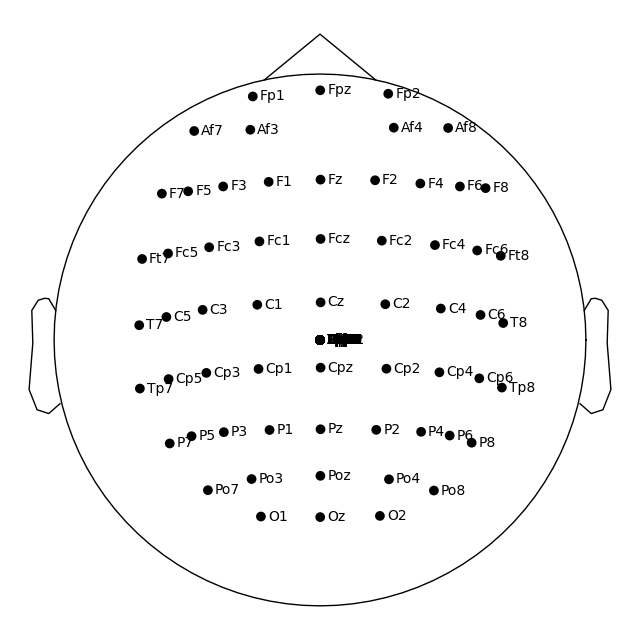
\includegraphics[width=0.9\textwidth]{images/BCI3IVa_Sensor_positions_(eeg).png}
%         \caption{Dynamic Bayes Network for Online SLAM. Source:\cite{Thrun98aprobabilistic}}
%     \end{figure}
%         The Pose information of the robot at time instant $t$ is represented as $x_t$ which constitutes $(x,y,\theta)$.
% where $(x,y)$ correspond to the location and $\theta$ represent orientation in the 2D Plane. Let $u_t$ be the Odometry reading of the motion executed between time $t-1$ and $t$. Let $Z_t$ be the LiDAR measurement taken at time $t$. Let $m$ be the Map created from the set of measurements. In figure \ref{fig:DBNOn}, the empty circles denote the states to be estimated and the shaded circles denote the variables that can be measured. Considering the circles to be the nodes and the arrows as edges, it is seen that the previous information on the state and the present command determines the current state of the system, which then influences the measurements obtained from map.The nodes $m$ and $x_{t+1}$ are the required output parameters. There are three basic fundamental approaches to the SLAM problem, namely, \textit{Kalman Filter}, \textit{Particle Filter}, \textit{Graph Network}. Each approach to the problem have their specific advantages and disadvantages, which will be discussed briefly in this chapter and extensively in upcoming chapters. However all the methods address the basic problem - Given the relative distance moved as recorded by the odometer and the observation at the current location, the system must be able to correctly localize and map its environment. In this chapter we will also look at how the probabilistic framework helps in achieving the task at hand and also the components commonly used across all the SLAM methods.
% %%%%%%%%%%%%%%%%%%%%%%%%%%%%%%%%%%%%%%%%%%%%%%%%%%%%%%%%%%%%%%%%%%%%%%%%%%%%%%%%%%%%%%%%%%%%%%%%%%%%%%%%%%%%%%
% \section{Probabilistic approach to state estimation}
%     In solving the \textit{online SLAM} Problem, the joint posterior distribution over the current pose and the map is the actual state of interest.
% \begin{equation} \label{eq:OnlSLM}
%     p(x_t, m | z_{1:t}, u_{0:t-1})
% \end{equation}
% whereas to solve the \textit{full SLAM }problem, the joint posterior distribution over  all the poses the robot had traversed and the map is the actual state of interest.
% \begin{equation} \label{eq:FullSLM}
%     p(x_{1:t}, m | z_{1:t}, u_{0:t-1})
% \end{equation}
% The distributions \ref{eq:FullSLM} and \ref{eq:OnlSLM} are applicable only to the grid based mapping because for Feature-based mapping the correspondence between the landmark measured and the measurement needs to be established and it is not estimated by the distributions mentioned above. This is a data association problem and it could be estimated as a part of the posterior distribution.
% \begin{equation} \label{CorresSLM}
%     p(x_{1:t}, m, c_t | z_{1:t}, u_{0:t-1})
% \end{equation}
% As this work is applicable only to grid-based mapping, Henceforth the derivations and equations are with respect to it without being mentioned explicitly.
% Applying the Bayes rule to determine the joint posterior distribution 
% \begin{equation} \label{eq:FullSLMc}
%     p(x_{1:t}, m | z_{1:t}, u_{0:t-1}) = \alpha . p(z_t | x_t, m).\int p(x_t| x_{t-1}, u_{t-1}). p(x_{1:t-1}, m | z_{1:t-1}, u_{0:t-2}) dx_{1:t-1}
% \end{equation}
% \par

% %EKF SLAM
% However estimating the states using \ref{eq:OnlSLM} becomes computationally expensive when integrating over all the previous poses and observation. This could be overcome by use of Extended KalmanFilter under three assumptions \textit{Feature-Based Maps} such that the number of landmarks are less , \textit{Gaussian Noise Assumption} such that the noise levels in the robot motion and perception is in limits that does not disturb the linearization of EKF and \textit{ Positive Information} such that unseen landmarks do not influence the estimation. In many practical applications the correspondence of a landmark to the measurement is not known. In such cases data association has to be derived during run time. In such cases, the correspondence is also estimated in the posterior distribution as shown in \refeq{eq:FullSLMc}.

% In the online SLAM process , as the robot moves through the environment, the system state vector and the covariance matrix are updated upon new measurements. 
% On observing new landmarks, new state variables are added to the system state vector and the covariance matrix. The EKF involves State Prediction and Correction step for every time a new information is received. The State Prediction and Correction steps are elaborated in subsequent sections. However the EKF has its own limitations. First, the covariance matrix maintained by the KalmanFilter has $K^2$ elements, where K is the number of landmarks. Hence the computational complexity rises to ${O}(K^2)$. Thus an increase in the number of the landmarks results in longer sensor updates. Second, The correspondence of the measurement and the landmarks is assumed to be known. Any wrong data association leads to filter divergence.  \par
% %RBPF SLAM
% Overcoming the problem, Rao-Blackwellized Particle Filters were used as a effective means to estimate the full posterior distribution. Instead of working on the entire distribution, particles were sampled at random and with sufficient number of particles the entire distribution could be covered.Here it is possible to relax the Gaussian assumption made in the EKF SLAM ,as any arbitrary distribution could be modelled as the target distribution. It basically involves steps such as Sampling, Importance Weighting, Re-sampling and Map Estimation. Sampling from proposal distribution corresponds to State prediction step and Importance Weighting corresponds to State Correction steps in EKF.
% More detailed discussion on RBPF is provided in the next chapter. This method is applicable to both Grid based and Feature Based mapping with fewer modifications.\par
% % %Graph SLAM
% % The third category of SLAM ...

% %%%%%%%%%%%%%%%%%%%%%%%%%%%%%%%%%%%%%%%%%%%%%%%%%%%%%%%%%%%%%%%%%%%%%%%%%%%%%%%%%%%%%%%%%%%%%%%%%%%%%%%%%%%%%%

% \section{State Prediction}
% State prediction is the key component in predicting the motion of the robot in case of EKF and Filter based SLAM methods, also it helps in creating the graph in front-end of graph based SLAM.The mobile robot is assumed to be equipped with odometer which provides relative motion of the wheels between time instances and a LiDAR sensor which can perceive the environment.Consider the positional state of the robot $x_{t-1}$ at time $t-1$, when subject to motion command $u_{t-1}$ the robot takes a new positional state $x_t$. The change in the positional state of the robot can be determined by use of motion models derived from translational and rotational kinematics or by using odometers. In equation \ref{eq:FullSLM}, the conditional density $p(x_t| x_{t-1}, u_{t-1})$ denote the state prediction part of the equation which could be replaced with appropriate motion models to predict the state of the robot in motion.The motion models derived will also need to factor the noise and uncertainty in its prediction, this is captured in the process noise covariance matrix. 

% \subsection{Odometry Motion Models}
% The odometers are basically wheel encoders which reads how much the wheels have moved through the environment on receiving the command. Hence it can only provide motion information post-the-fact, i.e. on receiving the motion command, the robot executes the command and then the odometry information is obtained. In many practical scenarios the robot might not follow all the motion commands as instructed due to slippage, wear and tear or due to any external forces. Under any such circumstances the odometer 
% provides much reliable information on the state of the robot. However 
% in case of motion planning this behaviour is not beneficial as the pose information at the next instance is critical to create a motion plan. In such cases the kinematic model of the 
% robot is used to predict the motion of the robot. 
% Algorithm for state prediction using odometry based motion model is very widely used in many robotics applications. Algorithms presented in the book \cite{Thrun98aprobabilistic} can be used off-the-self 
% for motion estimate implementation with odometry.
% On the downside, it is very common to observe drift and slippage in the odometer information and yet,it is most widely used in many robotics and industrial applications.

% \subsection{Kinematic Motion Models}
% In applications such as motion planning the positional state of the robot is required to be know in advance for planning and control. Depending on the number of tractions, dimensions of the robot the kinematic equations of the motion can be used to estimate the state of the system. \cite{R.Schubert} provides a detailed study on many different motion models which falls largely under the linear and curvilinear models. Linear motion models assume only straight motions and do not take rotations into account, whereas the curvilinear models assume the robot takes a circular path at a constant radius only exception being \textit{Constant Turn  Radius and Acceleration(CTRA)} which assumes that the robot follows a clothoid. The Figure \figurename{MtnMdl.png} provides the relationship and assumptions made by each of the motion models. \cite{R.Schubert}'s experiment results prove that curvilinear models provide better performance than linear models. Further CTRA shows better tracking results than the other curvilinear models. In \cite{Polack}, similar studies were made comparing Kinematic Bicycle Model and Dynamic models with 9-DOF, it was found that the earlier models were comparable to the dynamic model at low speeds and low angular acceleration. However at higher speeds or lateral
% acceleration ,the dynamic models with higher degrees of freedom were able to accurately plan the trajectory. Simplifying the solution to the problem and considering the theoretical  evidence in the literature, CTRA Motion Model is chosen as the motion model for state prediction in this thesis. The motion models derived are in continuous domain and these need to be discretized before it could be implemented on a computer. Methods such as Euler discretization or analytical methods are some of the common methods used in deriving discrete time representation of the process model and process covariance matrix. \cite{D.Svensson} provides the derivation of the discrete time equations for the CTRA model along with the process noise covariance modeled. The states involved in the prediction are longitudinal position ($x(t)$), lateral position ($y(t)$), heading angle ($\phi(t)$), speed ($s(t)$), acceleration ($a(t)$) and yaw rate ($\omega(t)$). In continuous domain the prediction function is derived and the discrete time model is derived using linearized discretization approach. The prediction equations are given by 
% \begin{gather} \label{CTRA_pred_ct}
%     x_{k+1}^{CTRA}
%     =
%     \begin{bmatrix} 
%         x_k \\ y_k \\ s_k \\ \phi_k \\ a_k\\ \omega_k
%     \end{bmatrix}
%     +
%     \begin{bmatrix} 
%         \Delta x_k \\ \Delta y_k \\ a_k T \\ \omega_k T \\ 0 \\ 0
%     \end{bmatrix}
%     + v_k
% \end{gather}
% where $T$ is predicition time and $v_k \thicksim  \mathcal{N}(0,Q_{k}^{CTRA})$ is the discrete time process noise that is a zero mean Gaussian noise with covariance $Q_k^{CTRA}$. For the complete derivation of the prediction function and the 
% process covariance matrix refer to \cite{D.Svensson}.

% %%%%%%%%%%%%%%%%%%%%%%%%%%%%%%%%%%%%%%%%%%%%%%%%%%%%%%%%%%%%%%%%%%%%%%%%%%%%%%%%%%%%%%%%%%%%%%%%%%%%%%%%%%%%%%
% \section{State Correction}
% The state of the system predicted using the motion models may not accurately define the state and its variance modeled using the process covariance matrix. In order to further deteremine 
% the exact posterior distribution, a confidence or a correction factor is required upon the predicted state. State correction techniques help in achieving a confidence or correction factor which helps in extracting precise information about the state predicted using the motion model. Various observation or measurement models can be chosen based on the sensor configuration present in the robot. In equation \ref{eq:FullSLM}, the conditional density $p(z_t | x_t, m)$ denotes the state correction part of the equation which can be replaced with appropriate measurement models or scan matching algorithms to estimate pose with confidence. Given the map $m$ and pose $x_t$ of the robot, the model must be able to summarise how the surrounding environment would seem to be. Numerous of research have been conducted on robot perception systems. Sensor systems such as LiDAR, Cameras, ultrasonic, radar are commonly used in various robotic applications depending on the environmental conditions where the robot is deployed.

% \subsection{Observation Models}
% In case of LiDAR, it is safe to asssume that every beam is independent of each other, hence the noise parameters and the measurement errors can be individually modelled. The measurement model density can thus be written as 
% \begin{equation}
%     p(z_t | x_t, m)  = \Pi_{k=1}^k  p(z_t^k | x_t, m)
% \end{equation}
% where  $z_t^k$ corresponds to a single laser beam. The density $p(z_t^k | x_t, m)$ can be modelled using different algorithms. Genrally it is a mixture of four distribution- Gaussian distribution at the incidence of an obstacle, exponentially decaying distribution to model unexpected objects in the view of actual obstacle, uniform distribution at the maximum range of laser beam and a uniform distribution throughout the range to include all unexpected measurements. The estimated value of the true measurement can be derived through ray casting operations in case of beam based models or nearest neighbour function in case of likelihood fields model\cite{Thrun98aprobabilistic}.  Algorithms suggested in the book \cite{Thrun98aprobabilistic} can be used off-the-shelf for estimating the ditribution.

% \subsection{Scan Matching}
% With advancement in computing power and use of LiDAR for perception it is possible to obtain more reliable results by registering two scans taken at two different relatively close poses and extract the relative poses between the two scans. This process of matching two scans is termed Scan Matching and it has been widely used for various applications. In other words, it is the method of finding the corrrect pose of the robot within a 3 dimensional search space which could provide the maximum value for the density $p(z_t | x_t, m)$. 
% \begin{equation}
%     \hat{x} _{t} = argmax_{x} p(x|m_{t-1}, z_t, x_t)
% \end{equation}
% \par
% Scan Matching is the core of this thesis. It will be discussed elaborately in subsequent chapters.

% \section{Summary}